\begin{minipage}{0.6\textwidth}
    \begin{figure}[H]
        \setcounter{figure}{13}
        \centering
        \includegraphics[width=0.9\columnwidth]{img/1.png}
        \caption{}
    \end{figure}
    то все они пересекутся в одной точке, над которой велась съемка. В правильных калейдоскопах вдоль этих линий изображения сливаются, в неправильных на них появляется «излом».
    \titleformat{\section}{\filcenter}{}{}{}
    \section*{Упражнения}
    \begin{enumerate}

        \setcounter{enumi}{8}
        \item Образует ли пара параллельных зеркал «правильный калейдоскоп» (хотя он и не подходит под наше определение калейдоскопа, можно проверить, удовлетворяет ли эта оптическая система определению правильности, данному выше)?
        \item Каково максимальное число изображений одной точки можно увидеть в двух зеркалах, поставленных под углом $\alpha$ друг к другу, если $\frac{180^\circ}{\alpha} = r$ и а) \textit{r} -- целое; б) \textit{r} -- не целое?
        \item Опять два зеркала образуют угол $\alpha$. Каково наибольшее число точек фундаментального «двуугольника» (угла), изображения которых можно увидеть в некоторой фиксированной точке А картинной плоскости такого калейдоскопа, меняя точку наблюдения? Изображения скольких точек фундаментального многоугольника накладываются в точке А с точки зрения геометрии? Рассмотрите три случая: $\alpha = \frac{180^\circ}{r}$ и а) \textit{r} -- иррационально; б) $r= \frac{p}{q}$ (несократимая дробь), $q \neq 1$; в) \textit{r} - натуральное число.
        \item Что видно в «цилиндрический калейдоскоп», если глаз расположить на оси цилиндра?
        \item Два плоских зеркала расположены под углом $40^\circ$ друг к другу. Какое максимальное число отражений светового луча возможно в этой оптической системе?
        \item В задаче 7 есть решение $n_1 = \infty$, $n_2 = 2$, $n_3 = 2$ ($\frac{180^\circ}{\infty}$ мы считаем равным нулю). Какому «калейдоскопу» соответствует это решение (каков физический смысл этого решения)?
    \end{enumerate} 
\end{minipage}
\indent
\begin{minipage}{0.3\textwidth} % Ширина второй колонки
    \titleformat{\section}{\filcenter\Large\bfseries}{}{}{}
    \section*{ОПИСАННАЯ ТРАПЕЦИЯ И СРЕДНИЕ}
    Взгляните на рисунок. Описанная трапеция, в которой проведены высота \textit{BH} и отрезок 4, перпендикулярный стороне \textit{AB}. Казалось бы, ничего особенно примечательного в этой фигуре нет, однако этот чертеж обладает удивительным свойством. На нем вместе с верхним основанием а и нижним основанием в уже содержатся все три средние этих отрезков: среднее арифметическое, сред нее геометрическое и среднее гармоническое, а именно:\[AB = \frac{a+b}{2},\] \[\quad BN = \sqrt{ab},\] \[\quad BG = \frac{2}{\frac{1}{a}+\frac{1}{b}}.\]
    Попробуйте самостоятельно доказать эти утверждения.
    \begin{figure}[H]
        \setcounter{figure}{13}
        \centering
        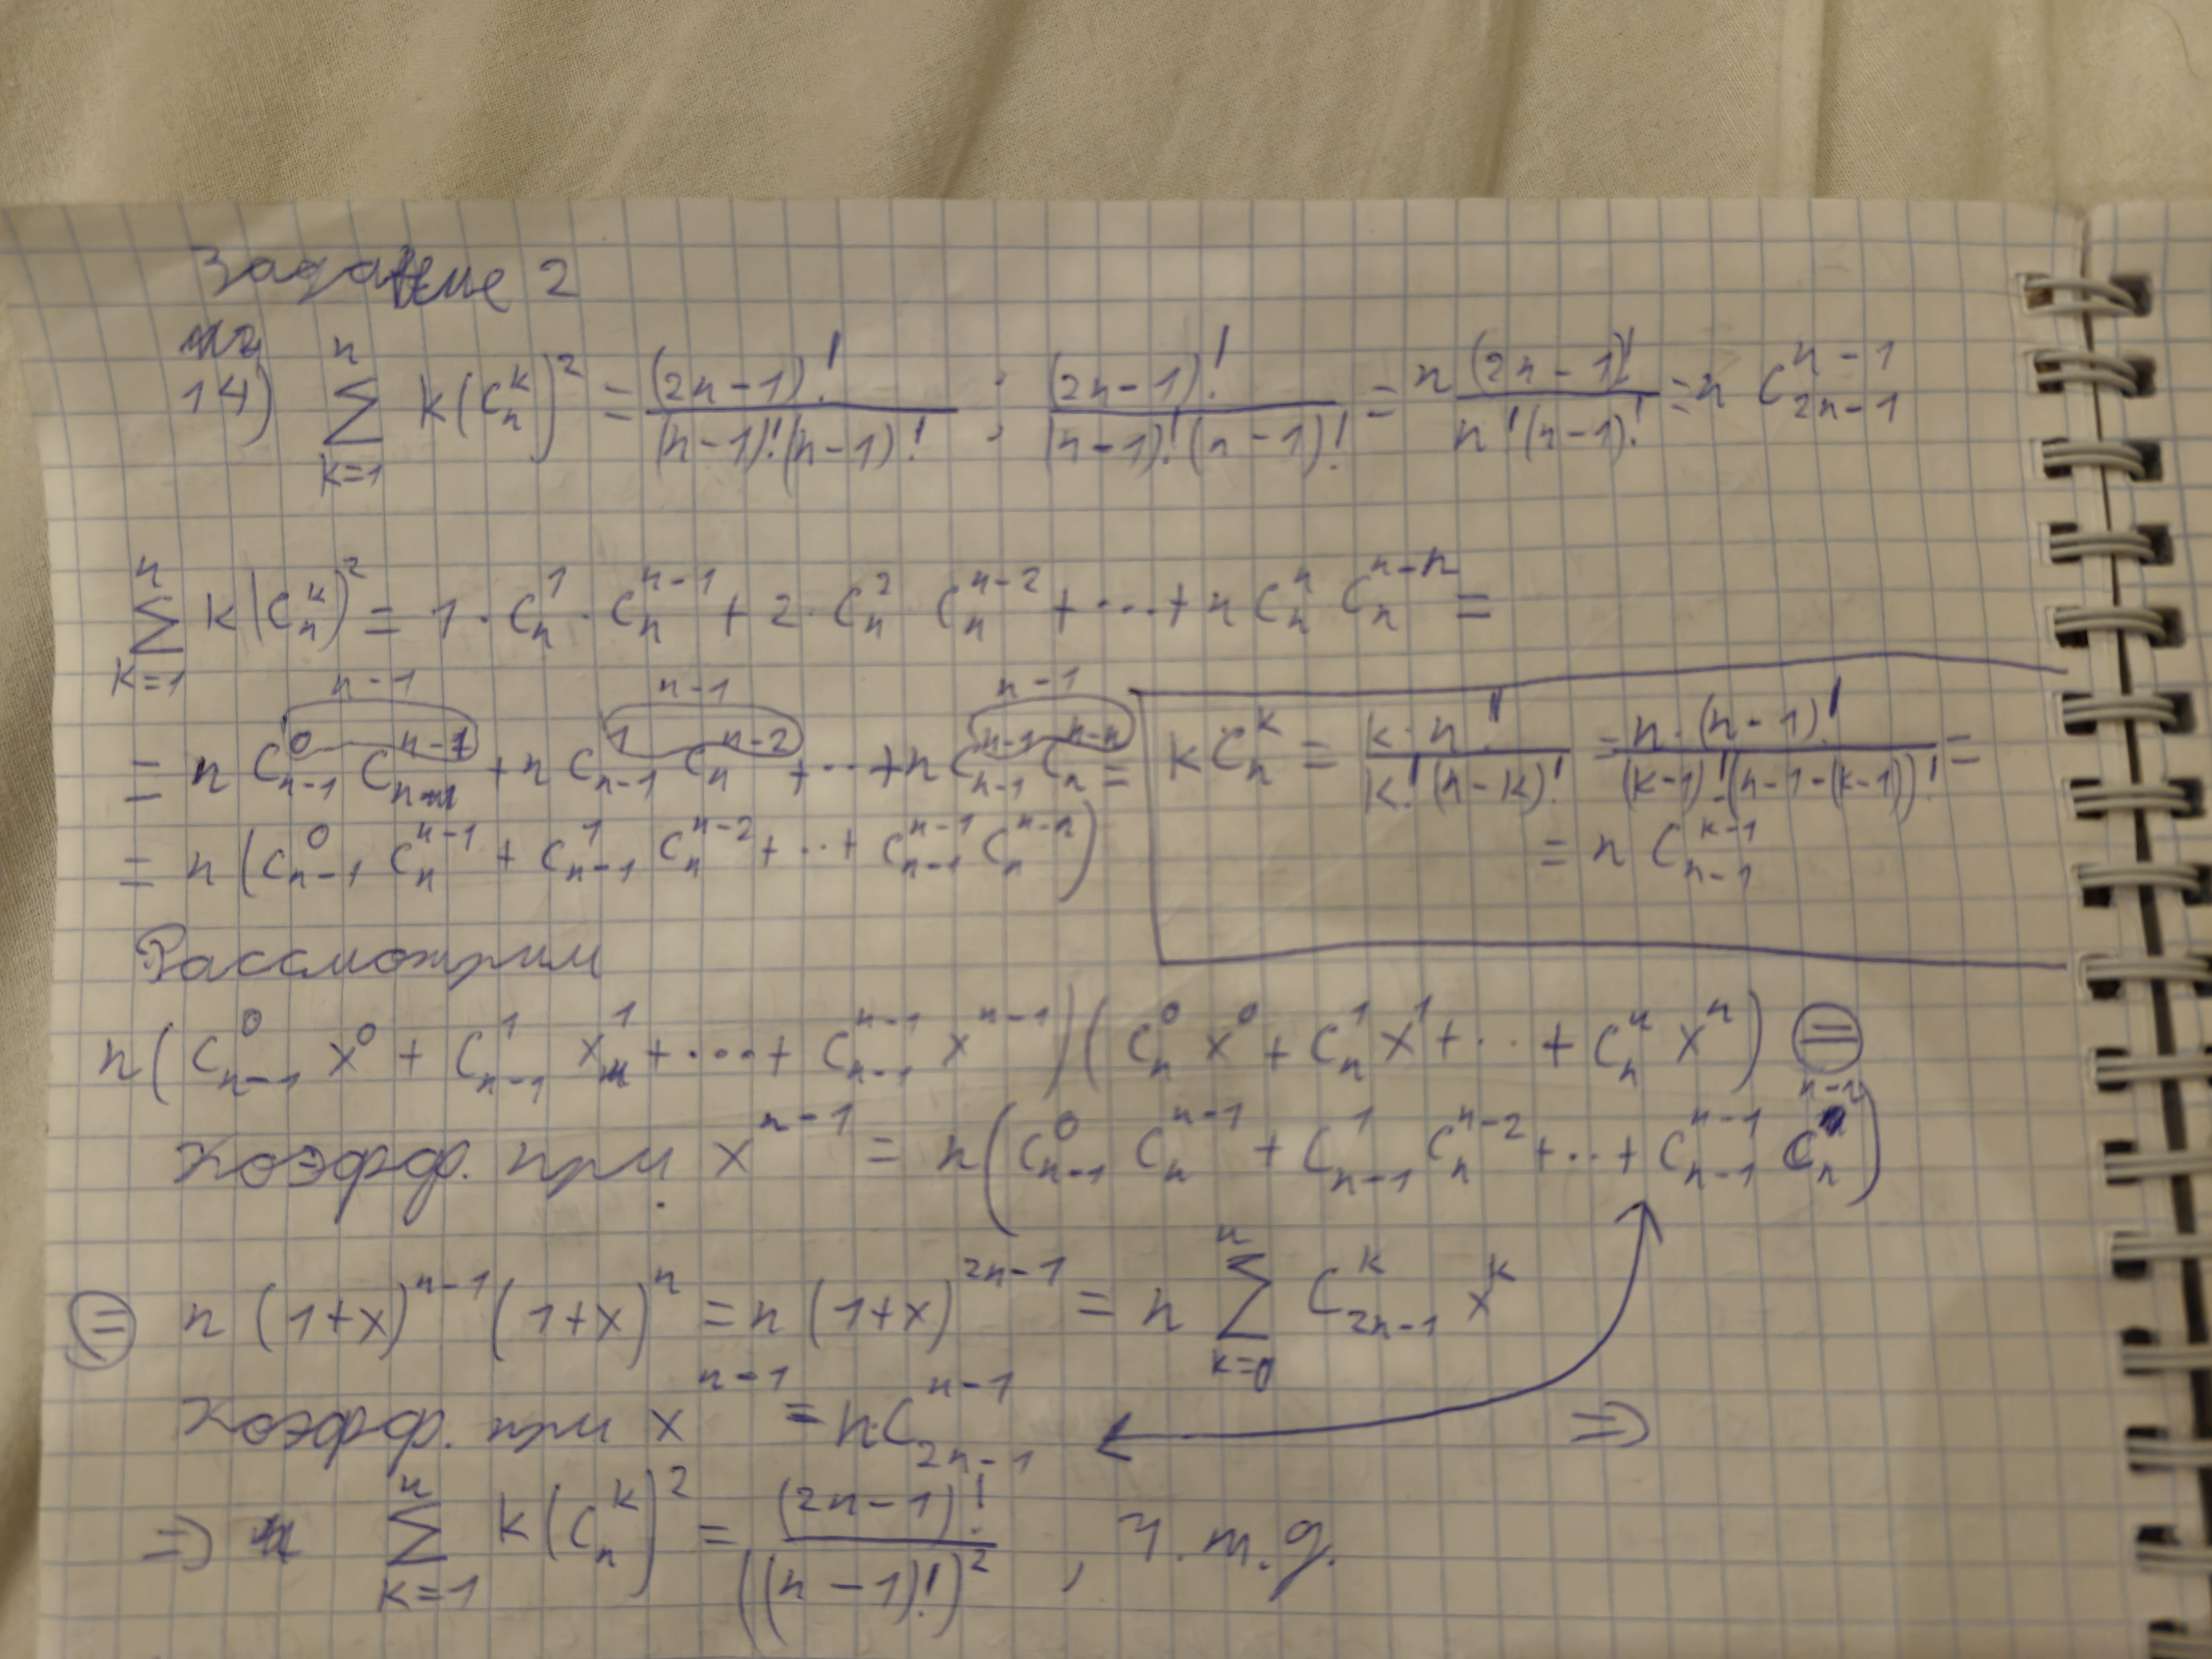
\includegraphics[width=1\columnwidth]{img/2.png}
    \end{figure}
    А теперь достаточно одного взгляда на чертеж, чтобы убедиться, что между средними выполнены следующие соотношения:
    \[ \frac{a+b}{2} \geq \sqrt{ab} \geq \frac{2}{\frac{1}{a}+\frac{1}{b}}.\]
    Действительно, \textit{AB} и \textit{BH} являются наклонной и перпендикуляром, проведенным к прямой \textit{AD} из точки \textit{B}, а \textit{BH} и \textit{BG} -- наклонная и перпендикуляр из точки \textit{B} к прямой \textit{HG}.\\
    
    {\textit{А. Савин, В. Сендеров}}\raggedleft
\end{minipage}
\begin{center}
    \begin{tabular}{|l|c|c|c|c|c|c|c|c|c|c|c|c|c|c|c|c|c|c|}
        \hline
        $n$ & 3 & 4 & 5 & 6 & 7 & 8 & 9 & 10 & 11 & 12 & 13 & 14 & 15 & 16 & 17 & 18 & 19 & 20  \\ 
        \hline
        $P(n)$ & 3  & 5 & 7 & 8 & 10 & 11 & 13 & 14 & 15 & 17 & 18 & 19 & 20 & 21 & 23 & 24 & 25 & 26 \\ 
        \hline
        $I(n)$ & 3  & 5 & 7 & 9 & 10 & 11 & 13 & 14 & 16 & 17 & 18 & 19 & 20 & 21 & 23 & 24 & 25 & 26 \\ 
        \hline
        $Q(n)$ & 4  & 5 & 8 & 9 & 10 & 11 & 14 & 15 & 16 & 17 & 18 & 19 & 20 & 21 & 24 & 25 & 26 & 27 \\ 
        \hline
    \end{tabular}
\end{center}
